\chapter{Experimental Results and Evaluation}

This chapter summarizes the experimental results from each stage. It first presents the frame-based vision results, then the offline RVT validation, and finally the real-time event pipeline. Detection accuracy, runtime, and topic output rate are different types of metrics, so they are reported separately and explained in the corresponding sections.

\section{Frame-Based Vision Results}

The frame-based vision stage mainly verified real-time object detection, simple object tracking, and the basic KITTI evaluation process on the Jetson. Several pretrained detection networks ran successfully on the Jetson, including SSD-MobileNet-v2, SSD-Inception-v2, PeopleNet, DashCamNet, and TrafficCamNet. Camera or image input could produce bounding boxes correctly, and the IoU tracking program could keep track IDs for detected objects across continuous frames. This shows that camera input, object detection, and the basic tracking program can run continuously on the Jetson.

The KITTI batch-processing program completed image loading, prediction saving, visualization, and ground-truth matching. It could match predicted boxes with ground-truth boxes, count TP, FP, and FN, and calculate Precision, Recall, and F1. Because this program does not implement all evaluation rules of the official KITTI benchmark, such as difficulty, DontCare, truncation, occlusion, and AP calculation, this report treats these results only as a basic detection evaluation.

The runtime test used the pretrained SSD-MobileNet-v2 model and processed 100 KITTI images. Before formal timing, a small number of images were used for warm-up to reduce the extra overhead of the first inference. The program uses \texttt{std::chrono} only around the \texttt{net->Detect()} call, so disk image loading and result saving are not included. This test measured an average \texttt{DetectNet} call time of 9.52411 ms per image, corresponding to 104.997 FPS. At the same time, \texttt{GetNetworkFPS()} reported an internal network speed of 154.128 FPS, which is about 6.49 ms per image.

The two results measure different parts of the process. The 104.997 FPS result corresponds to the complete \texttt{net->Detect()} call. In addition to the TensorRT network forward pass, it also includes image preprocessing, detection postprocessing, bounding-box parsing, synchronization, and other overhead. The 154.128 FPS value mainly represents the internal network-computation speed reported by Jetson-Inference. Therefore, this report uses about 105 FPS as the measured result for the \texttt{DetectNet} call and does not treat 154 FPS as the same metric.

\section{Offline RVT Detection Results}
\label{sec:rvt_results}

The offline RVT stage was used to confirm that the event-based object detection model could complete the full GEN1 validation on the Jetson and that the ported evaluation process worked correctly. The complete GEN1 validation finished successfully on the Jetson GPU. The main detection metrics are shown in Table~\ref{tab:rvt_gen1}.

\begin{table}[htbp]
\centering
\caption{Complete GEN1 validation results of RVT-Tiny on the Jetson.}
\label{tab:rvt_gen1}
\begin{tabular}{lc}
\toprule
Metric & Result \\
\midrule
mAP & 45.77\% \\
AP50 & 71.06\% \\
AP75 & 48.80\% \\
AP small (AP\_S) & 38.38\% \\
\bottomrule
\end{tabular}
\end{table}

The RVT evaluation program uses COCO-style object detection metrics~\parencite{rvtGithub}. mAP, AP50, and AP75 were introduced earlier. AP small, written as \texttt{AP\_S} in the code, only measures detection results for small objects. In the COCO definition, this means objects with a bounding-box area smaller than $32^2$ pixels. Therefore, these metrics show detection performance under different matching requirements or for different object sizes.

The complete validation used the RVT-Tiny GEN1 checkpoint with \texttt{batch\_size.eval=1}, \texttt{hardware.num\_workers.eval=0}, and a postprocessing confidence threshold of \texttt{0.001}~\parencite{rvtGithub}. The validation ran for 18714 iterations with a total runtime of 1:46:10 and an average speed of about 2.94 iteration/s. The complete runtime also includes data loading, postprocessing, NMS, evaluation, and other steps, so it cannot be directly treated as the single-inference latency of the model. The original RVT paper reports about 47.2\% mAP on GEN1~\parencite{gehrig2023}, while this project obtained 45.77\% AP on the Jetson.

The modified visualization program can generate comparison images of predictions and ground-truth annotations. These images are used to observe missed detections, false detections, bounding-box positions, and prediction changes under different confidence thresholds. A lower confidence threshold shows more low-confidence prediction boxes, while a higher threshold makes the images clearer for manual observation.

Figure~\ref{fig:rvt_offline_results} shows three groups of offline RVT-Tiny detection examples based on the GEN1 dataset. GEN1 is the event dataset used for the offline RVT validation, so these results are also the GEN1 visualization results of this project. When predicted boxes are close to the ground-truth boxes, the object position predicted by the model can be checked directly. Differences between them can be used to observe missed detections, false detections, or localization errors.

\begin{figure}[htbp]
    \centering
    \begin{subfigure}[t]{0.32\textwidth}
        \centering
        \IfFileExists{images/rvt_offline_01.png}{
            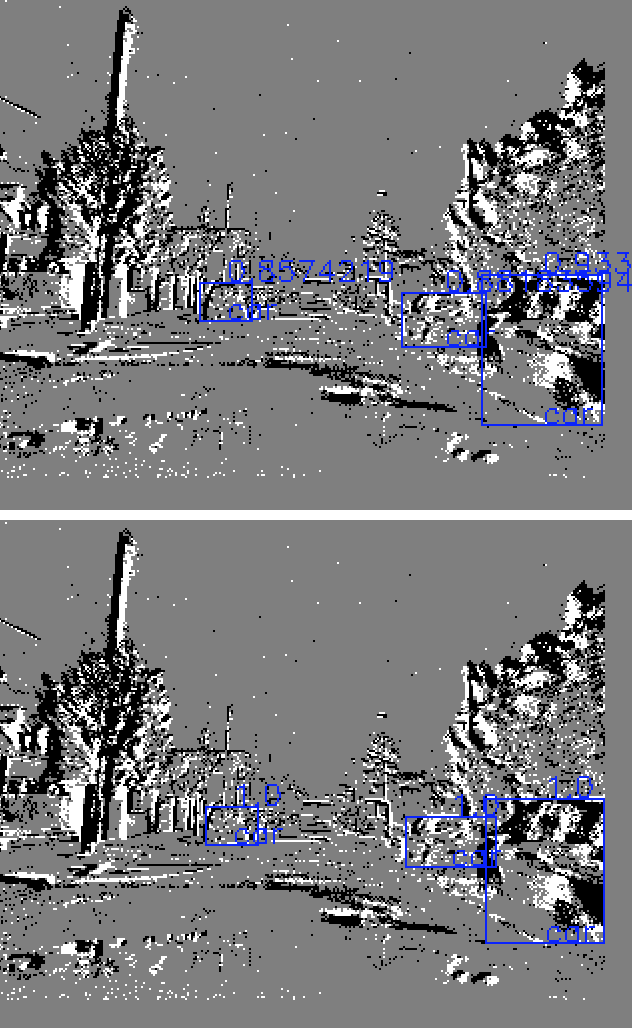
\includegraphics[width=\linewidth]{images/rvt_offline_01.png}
        }{
            \fbox{\parbox[c][0.16\textheight][c]{0.92\linewidth}{\centering \texttt{rvt\_offline\_01.png}}}
        }
        \caption{Example 1}
    \end{subfigure}
    \hfill
    \begin{subfigure}[t]{0.32\textwidth}
        \centering
        \IfFileExists{images/rvt_offline_02.png}{
            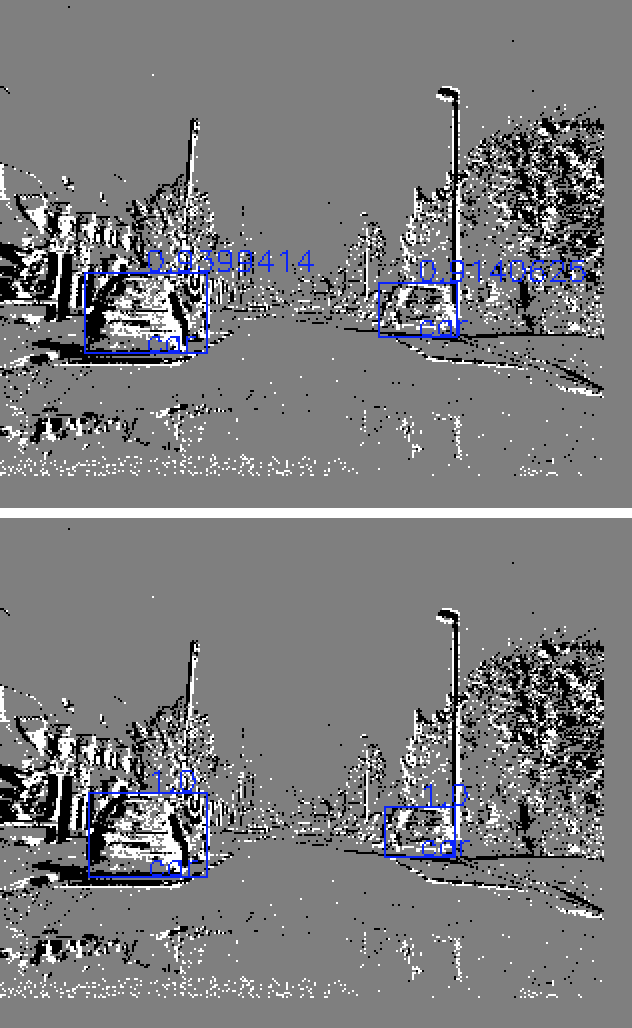
\includegraphics[width=\linewidth]{images/rvt_offline_02.png}
        }{
            \fbox{\parbox[c][0.16\textheight][c]{0.92\linewidth}{\centering \texttt{rvt\_offline\_02.png}}}
        }
        \caption{Example 2}
    \end{subfigure}
    \hfill
    \begin{subfigure}[t]{0.32\textwidth}
        \centering
        \IfFileExists{images/rvt_offline_03.png}{
            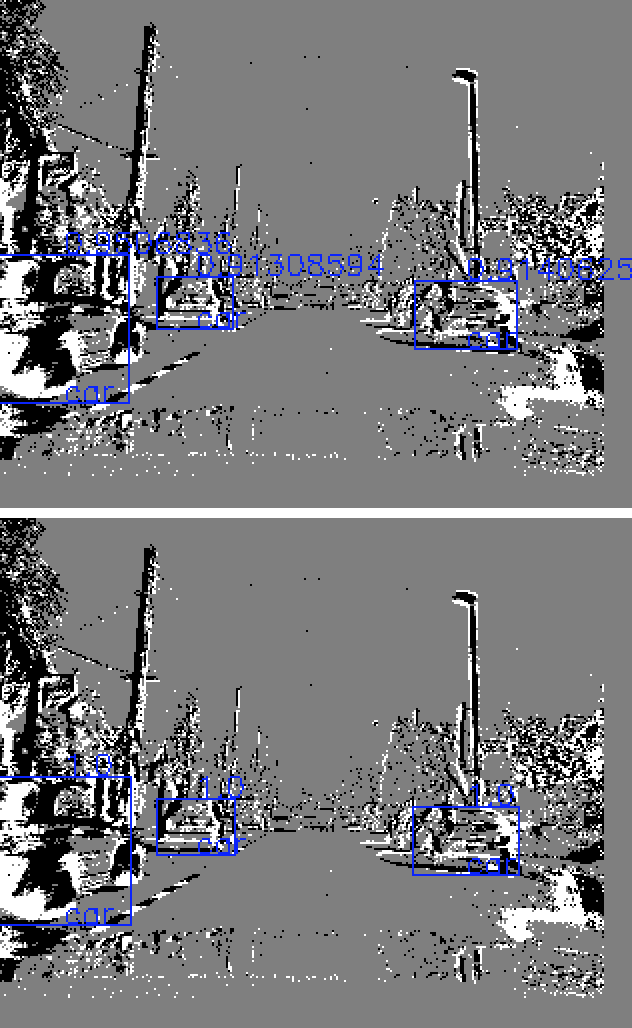
\includegraphics[width=\linewidth]{images/rvt_offline_03.png}
        }{
            \fbox{\parbox[c][0.16\textheight][c]{0.92\linewidth}{\centering \texttt{rvt\_offline\_03.png}}}
        }
        \caption{Example 3}
    \end{subfigure}
    \caption{Examples of offline RVT-Tiny predictions and ground-truth annotations on the GEN1 dataset.}
    \label{fig:rvt_offline_results}
\end{figure}

\section{Validation of the Final Real-Time Event Pipeline}
\label{sec:realtime_results}

The final real-time system was validated at three levels. First, the IMX636, the existing FPGA/V4L2 data path, and Metavision/OpenEB were checked to confirm that they could produce real event data. Second, the Kria was checked to confirm that it could continuously publish raw events as ROS 2 \texttt{EventPacket} messages and send them to the Jetson over Ethernet. Finally, \texttt{event\_camera\_codecs} and \texttt{event\_camera\_renderer} inside Jetson Docker were checked to confirm that they could decode and render the events and output images that could be displayed. The current final test configuration uses EVT3, and the event topic is \path{/metavision_driver/events}. In the physical test, ROS 2 topic queries confirmed that the renderer output image topic was \path{/metavision_driver/renderer/image_raw}, which was subscribed to and displayed by \texttt{rqt\_image\_view} on the Jetson host.

On the Jetson, \texttt{ros2 topic hz} was used to continuously measure \path{/metavision_driver/events}. In the experimental records, the observed \texttt{EventPacket} message rate during stable operation was mainly about 52--55 Hz. This rate represents the arrival rate of ROS 2 message packets, not the generation rate of individual events. The number of EVT3 events contained in each \texttt{EventPacket} can change with the scene.

\texttt{ros2 topic bw} was then used to measure the event-topic data rate actually received by the Jetson subscriber. In the experimental records, the observed throughput in normal dynamic scenes was mainly about 11.6--14.2 MB/s, and the average size of a single \texttt{EventPacket} was usually about 0.12--0.14 MB. When an object was moved quickly, the observed throughput increased to about 20 MB/s. After the camera was covered and the scene had little change, the throughput decreased to about 1.2--1.9 MB/s. This behavior shows the relationship between the amount of event data and the dynamics of the scene. In the actual tests, without software rate limiting, the 1 GbE transfer from the Kria to the Jetson showed clear stalling and data accumulation. Therefore, the current configuration sets the byte-rate limiter to 20,000,000 bytes/s and enables the event-rate controller at 5,000,000 events/s. As a result, about 20 MB/s is an observed value under the controlled configuration and should not be interpreted as the maximum unrestricted natural output bandwidth of the IMX636. It is also important to note that the value reported by \texttt{ros2 topic bw} is the ROS 2 message-data throughput observed on the subscriber side. It is not the same as the total physical-link bandwidth including DDS, UDP/IP, and Ethernet protocol overhead.

\begin{table}[htbp]
\centering
\caption{Observed data throughput of \path{/metavision_driver/events} in different scenes.}
\label{tab:event_topic_bandwidth}
\begin{tabular}{lc}
\toprule
Scene & Observed throughput \\
\midrule
Normal dynamic scene & about 11.6--14.2 MB/s \\
Fast-motion scene & about 20 MB/s \\
Low-change scene after covering the camera & about 1.2--1.9 MB/s \\
\bottomrule
\end{tabular}
\end{table}

According to the documentation of \texttt{event\_camera\_renderer}, the default value of the image publication parameter \texttt{fps} is 25 Hz~\parencite{eventCameraRenderer}. In the final test, the renderer log continuously reported an internal publication rate of about 25.00 Hz during stable operation. The delay values in the log were mainly about 24.8--25.8 ms. The Kria and Jetson currently do not use a common time reference, so there is a clock difference between the two devices. Therefore, this delay is affected by the time difference between the devices and cannot be directly interpreted as the real network latency or the strict end-to-end latency from sensor to display.

The final real-time display result is shown in Figure~\ref{fig:kria_jetson_rqt_final}. The image comes from a real IMX636 event stream after Kria publication, network transfer, and Jetson-side rendering. Therefore, it is mainly used to confirm that the complete data pipeline is connected. It shows the visualization result after event rendering.

\begin{figure}[htbp]
    \centering
    \IfFileExists{images/kria_jetson_rqt_final.png}{
        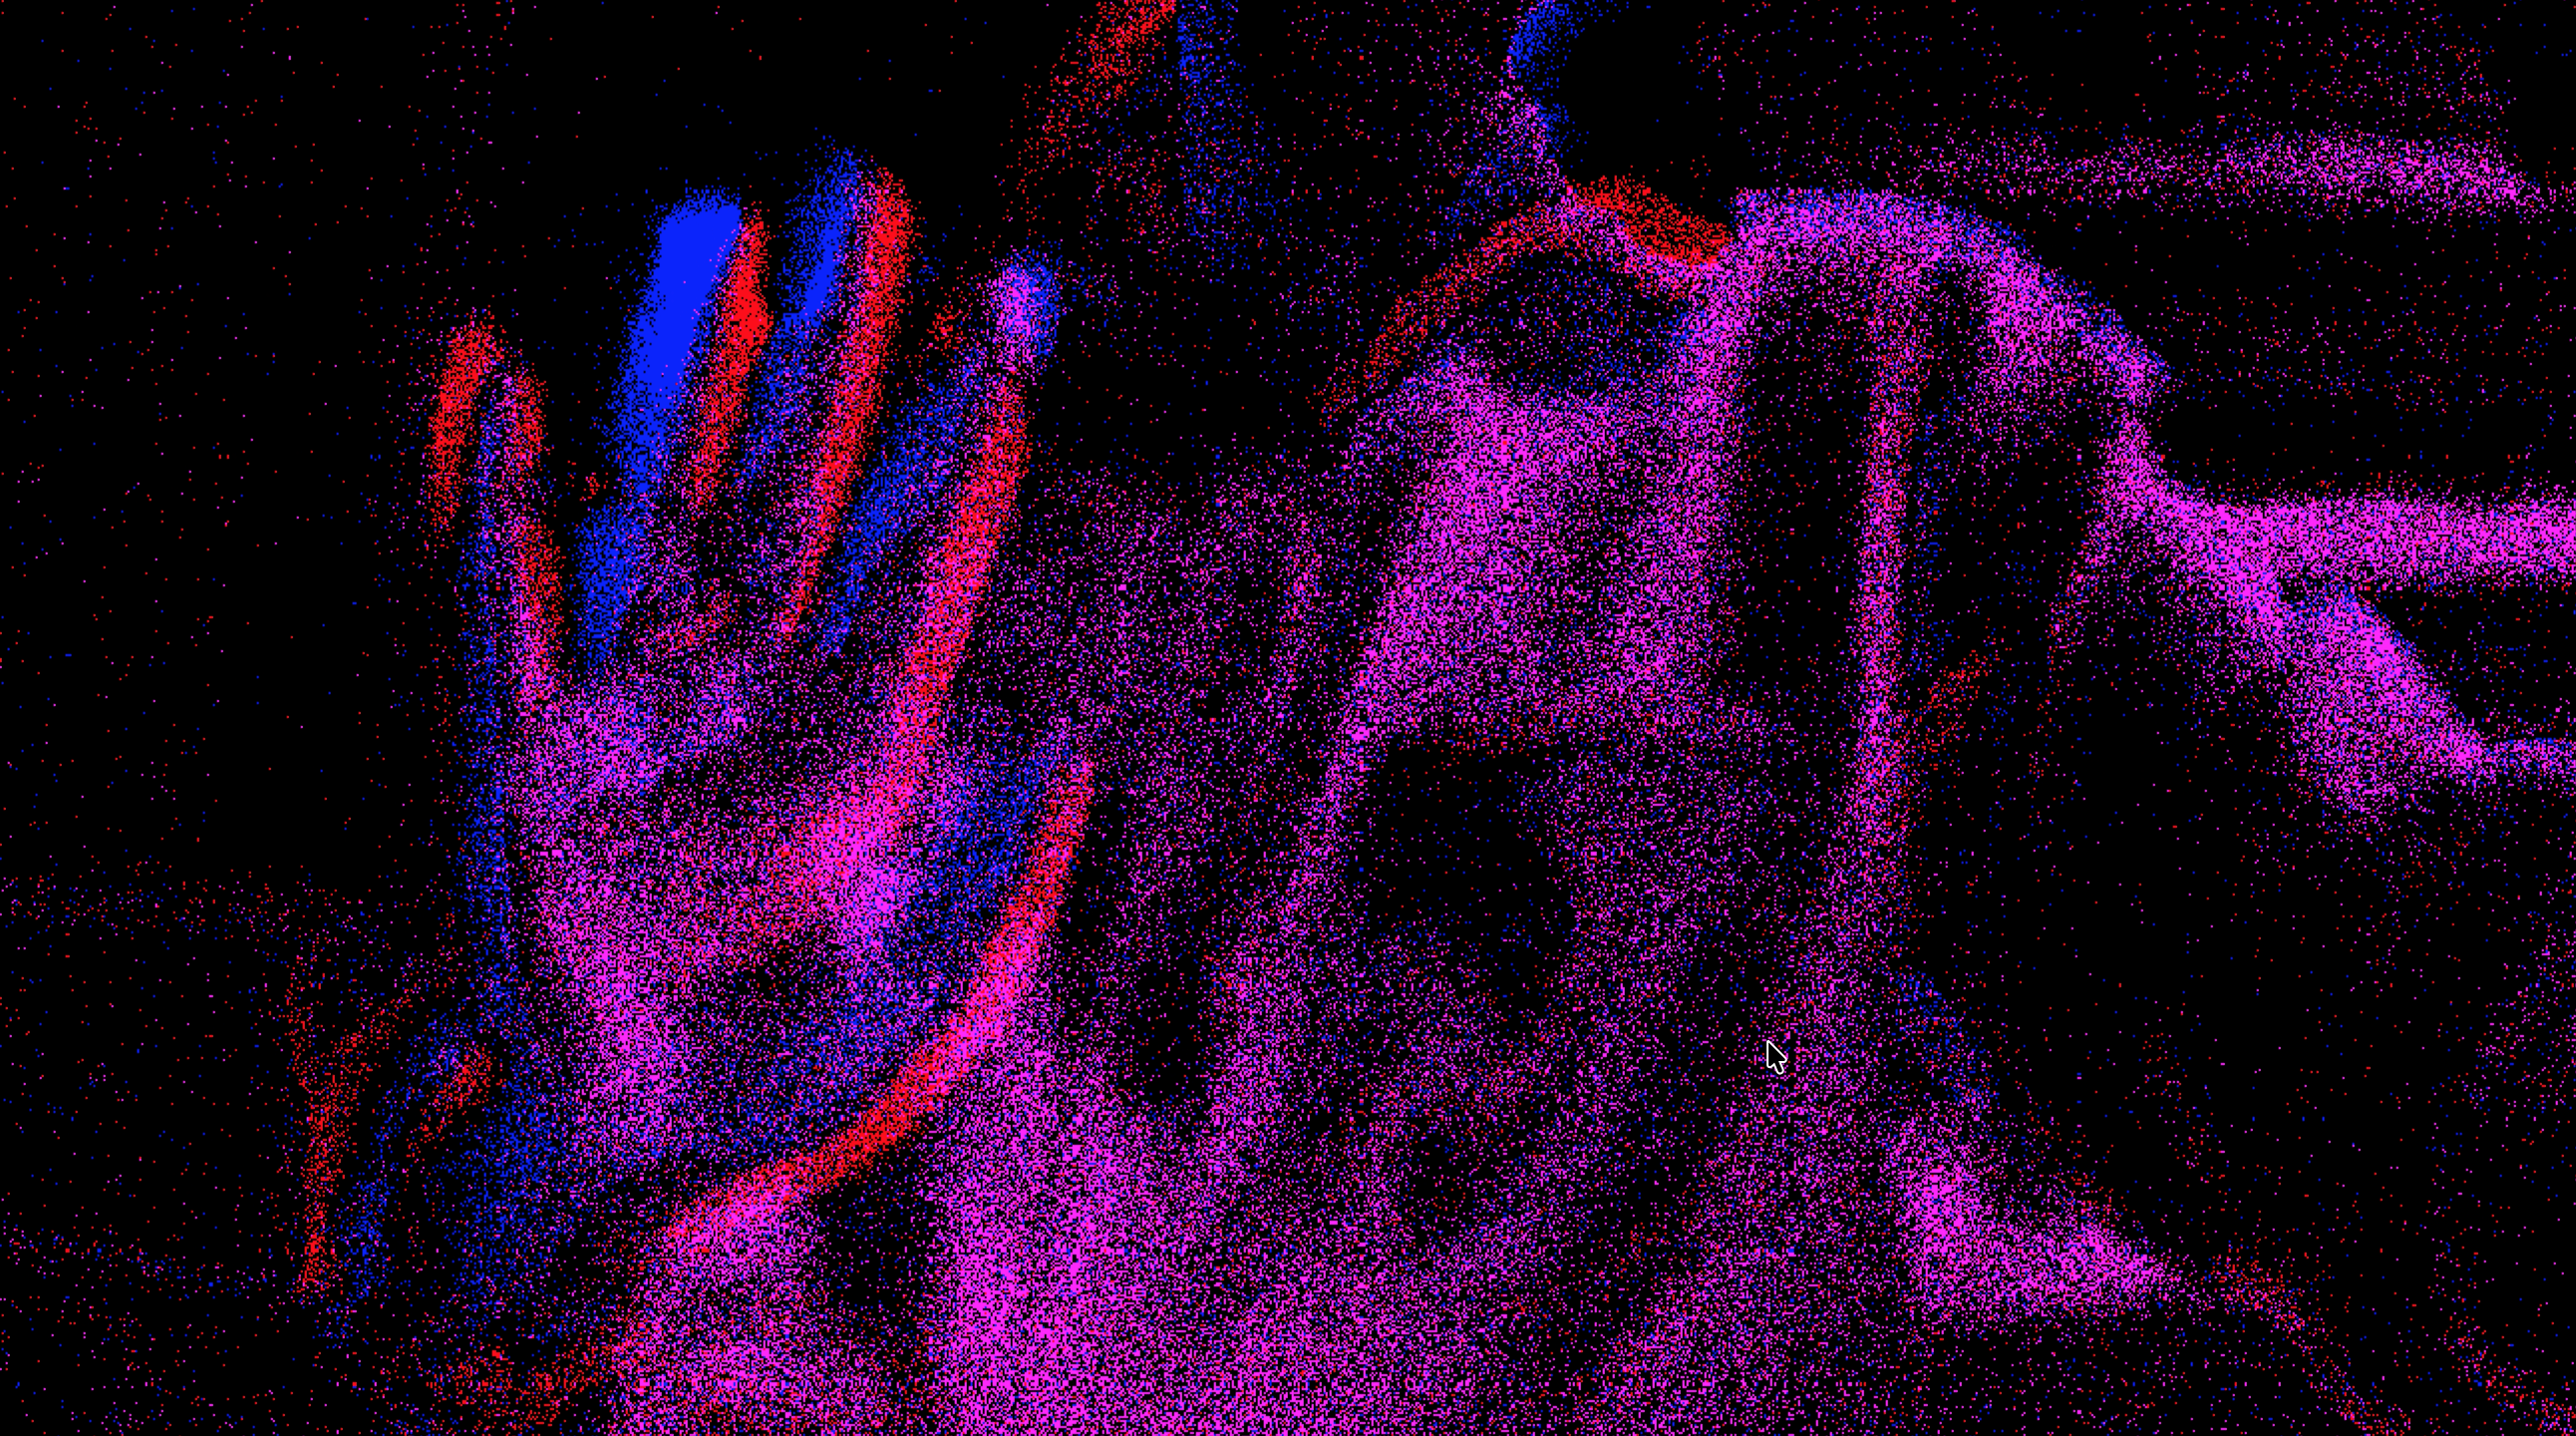
\includegraphics[width=0.9\textwidth]{images/kria_jetson_rqt_final.png}
    }{
        \fbox{\parbox[c][0.24\textheight][c]{0.84\textwidth}{\centering Image to be uploaded: \texttt{kria\_jetson\_rqt\_final.png}}}
    }
    \caption{Final display result of the real-time EVT3 processing pipeline between Kria and Jetson.}
    \label{fig:kria_jetson_rqt_final}
\end{figure}
